\section{How does the decline of HPV changes if the percentage of MSMs increases significantly?}

As we mentioned before, the data used in this work is a little bit old and the sexual behavior of the people has experimented changes in the last years. Thus, it would be interesting to perform some simulations adapting properly the model parameters. Here, we propose an increasing in the percentage of men who have sex with men (MSM).

In our proposal we have assumed that the percentage of MSM in the population is $3.88\%$. This value is provided by \cite{INE}. However, this survey was published in 2003. Then, here, we are going to increase the percentage of MSM from $3.88\%$ until $10\%$.  Only girls are vaccinated with a $70\%$ coverage (Spanish current program).

In Figure \ref{fig:compara_MSM} we can see graphically the obtained results. 

\begin{figure}[!]
	\centering
	\begin{tabular}{cc}
		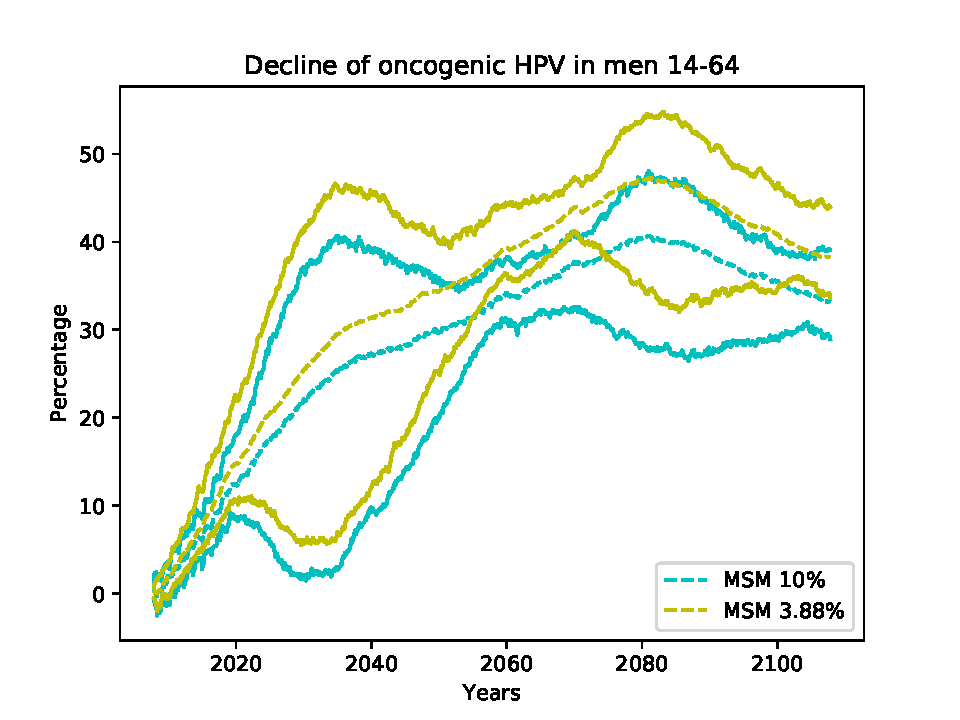
\includegraphics[width=0.5\linewidth]{IMGs/13.-Aumento_MSM/onco_hom.pdf}	& 
		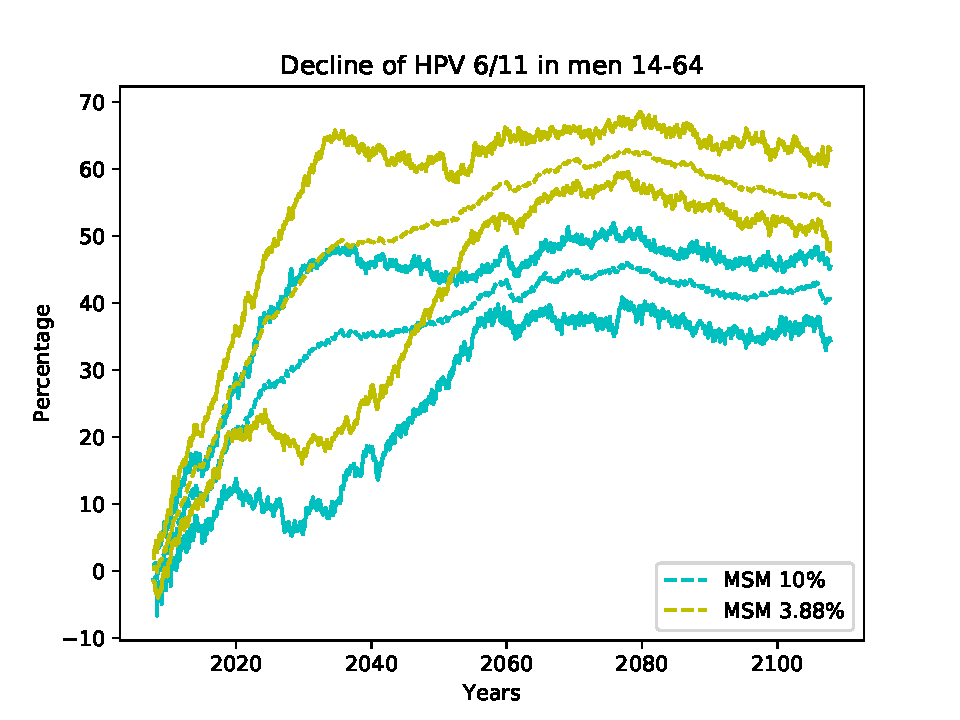
\includegraphics[width=0.5\linewidth]{IMGs/13.-Aumento_MSM/verr_hom.pdf}  \\ 
		Decline oncogenic HPV men	& Decline HPV 6/11 men \\ 
		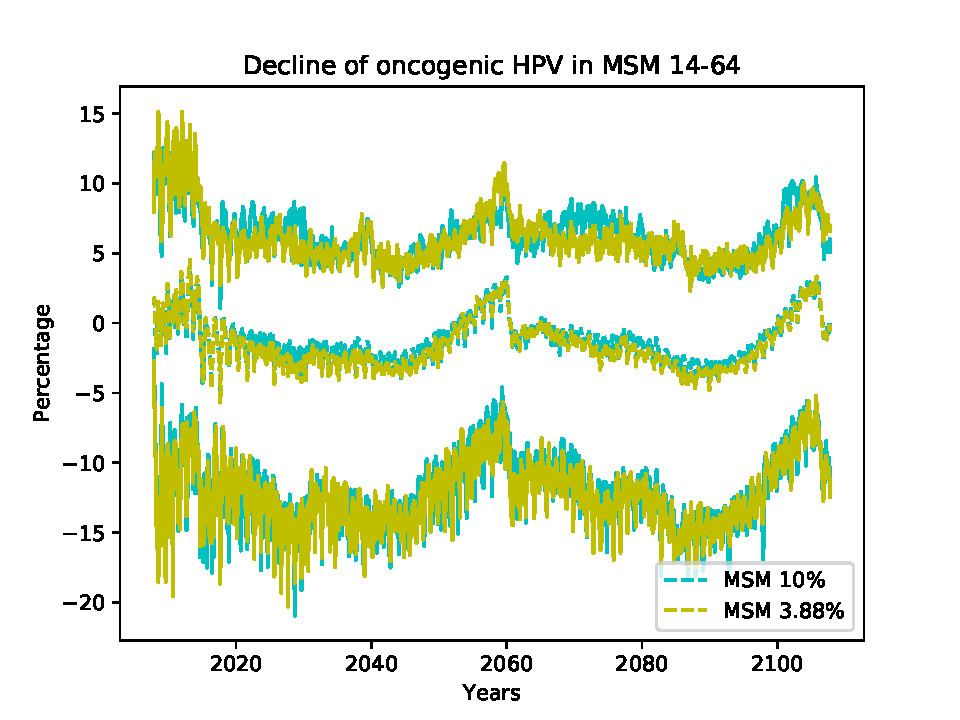
\includegraphics[width=0.5\linewidth]{IMGs/13.-Aumento_MSM/onco_MSM.pdf}	& 
		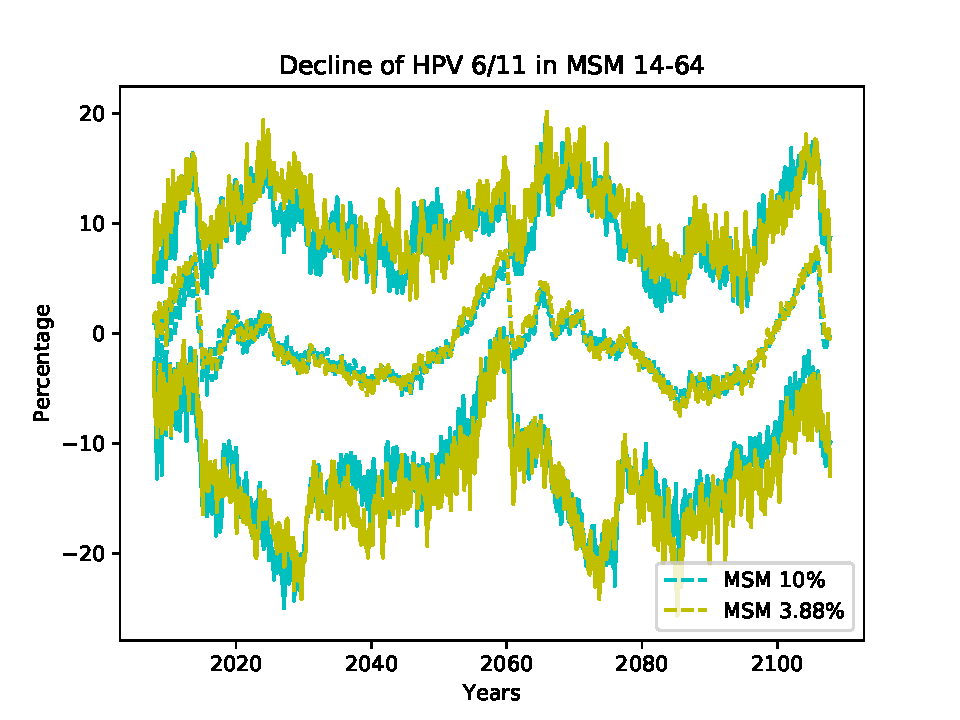
\includegraphics[width=0.5\linewidth]{IMGs/13.-Aumento_MSM/verr_MSM.pdf}  \\ 
		Decline oncogenic HPV MSM	& Decline HPV 6/11 MSM \\ 
		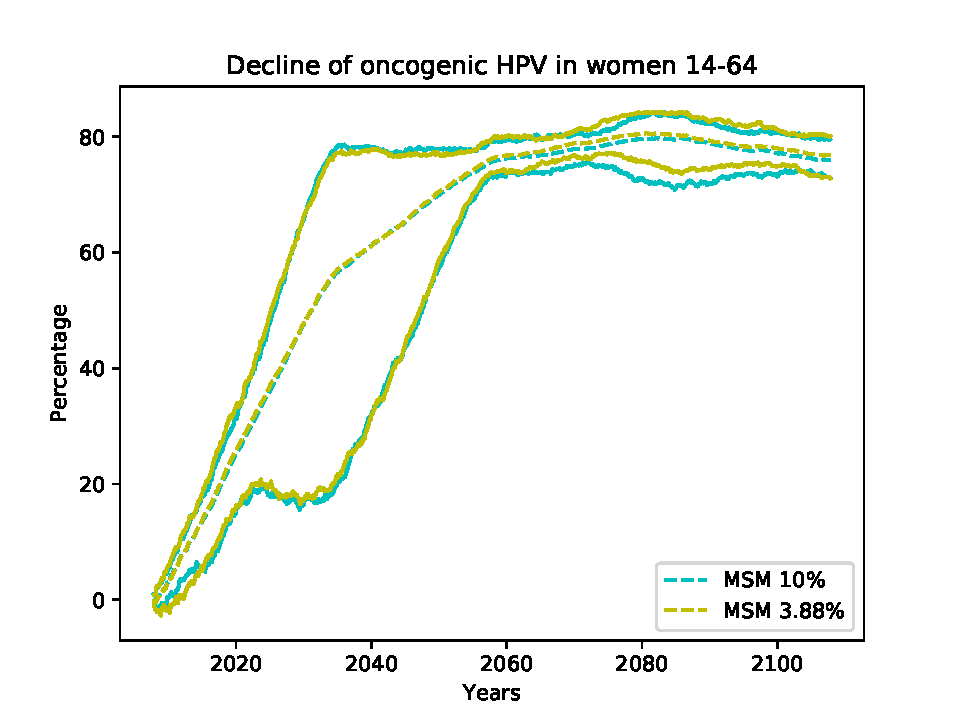
\includegraphics[width=0.5\linewidth]{IMGs/13.-Aumento_MSM/onco_muj.pdf}	& 
		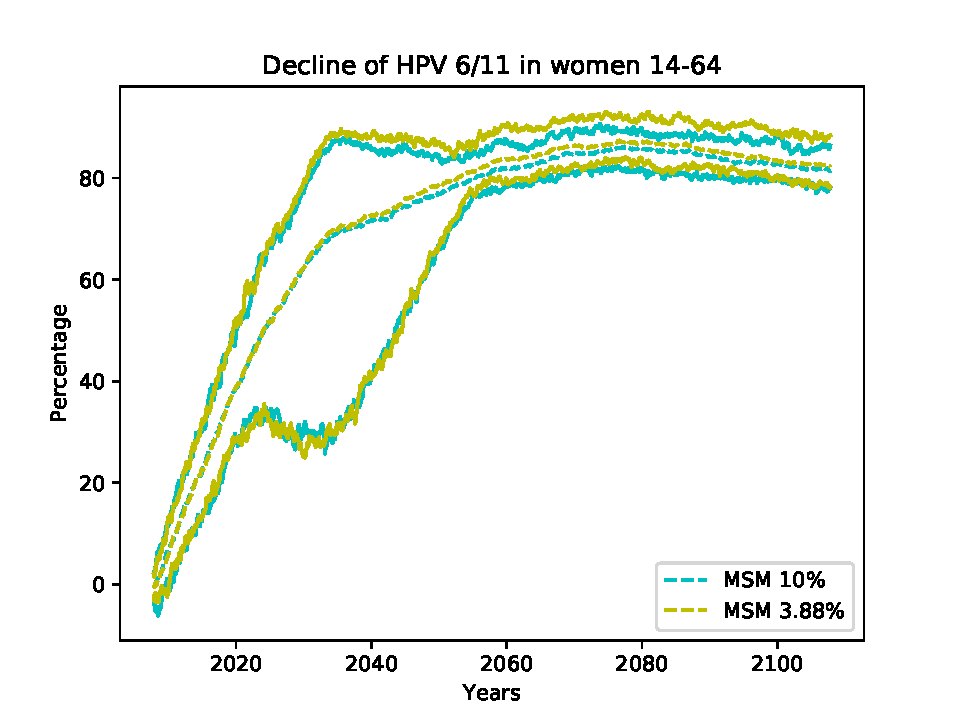
\includegraphics[width=0.5\linewidth]{IMGs/13.-Aumento_MSM/verr_muj.pdf}  \\ 
		Decline oncogenic HPV women	& Decline HPV 6/11 women \\ 
	\end{tabular} 
	\caption{Comparative of the decline of HPV in case the number of MSM increases from $3.88\%$ until $10\%$. In the current vaccination scenario (vaccinating only girls with a coverage of $70\%$, significant declines in oncogenic HPV in men and HPV 6/11 in men appear.}
	\label{fig:compara_MSM}
\end{figure}

As we can see, the decline does not change in MSM. The decline in women hardly changes, at most 2\% in the decline of HPV 6/11 in women. Nevertheless, in men, there is an average difference in the decline of oncogenic HPV about $4.6\%-7.0\%$ and $13.1\%-18.2\%$ in HPV 6/11.

As we mentioned before, this simulation can be considered as a sensitivity analysis to support the robustness of this study.
